% Options for packages loaded elsewhere
\PassOptionsToPackage{unicode}{hyperref}
\PassOptionsToPackage{hyphens}{url}
%
\documentclass[
  11pt,
]{book}
\usepackage{lmodern}
\usepackage{amssymb,amsmath}
\usepackage{ifxetex,ifluatex}
\ifnum 0\ifxetex 1\fi\ifluatex 1\fi=0 % if pdftex
  \usepackage[T1]{fontenc}
  \usepackage[utf8]{inputenc}
  \usepackage{textcomp} % provide euro and other symbols
\else % if luatex or xetex
  \usepackage{unicode-math}
  \defaultfontfeatures{Scale=MatchLowercase}
  \defaultfontfeatures[\rmfamily]{Ligatures=TeX,Scale=1}
  \setmainfont[]{Palatino}
  \setmonofont[Scale=0.8]{Source Code Pro}
\fi
% Use upquote if available, for straight quotes in verbatim environments
\IfFileExists{upquote.sty}{\usepackage{upquote}}{}
\IfFileExists{microtype.sty}{% use microtype if available
  \usepackage[]{microtype}
  \UseMicrotypeSet[protrusion]{basicmath} % disable protrusion for tt fonts
}{}
\makeatletter
\@ifundefined{KOMAClassName}{% if non-KOMA class
  \IfFileExists{parskip.sty}{%
    \usepackage{parskip}
  }{% else
    \setlength{\parindent}{0pt}
    \setlength{\parskip}{6pt plus 2pt minus 1pt}}
}{% if KOMA class
  \KOMAoptions{parskip=half}}
\makeatother
\usepackage{xcolor}
\IfFileExists{xurl.sty}{\usepackage{xurl}}{} % add URL line breaks if available
\IfFileExists{bookmark.sty}{\usepackage{bookmark}}{\usepackage{hyperref}}
\hypersetup{
  pdftitle={Investigación Social Abierta},
  pdfauthor={Juan Carlos Castillo},
  hidelinks,
  pdfcreator={LaTeX via pandoc}}
\urlstyle{same} % disable monospaced font for URLs
\usepackage{color}
\usepackage{fancyvrb}
\newcommand{\VerbBar}{|}
\newcommand{\VERB}{\Verb[commandchars=\\\{\}]}
\DefineVerbatimEnvironment{Highlighting}{Verbatim}{commandchars=\\\{\}}
% Add ',fontsize=\small' for more characters per line
\usepackage{framed}
\definecolor{shadecolor}{RGB}{248,248,248}
\newenvironment{Shaded}{\begin{snugshade}}{\end{snugshade}}
\newcommand{\AlertTok}[1]{\textcolor[rgb]{0.94,0.16,0.16}{#1}}
\newcommand{\AnnotationTok}[1]{\textcolor[rgb]{0.56,0.35,0.01}{\textbf{\textit{#1}}}}
\newcommand{\AttributeTok}[1]{\textcolor[rgb]{0.77,0.63,0.00}{#1}}
\newcommand{\BaseNTok}[1]{\textcolor[rgb]{0.00,0.00,0.81}{#1}}
\newcommand{\BuiltInTok}[1]{#1}
\newcommand{\CharTok}[1]{\textcolor[rgb]{0.31,0.60,0.02}{#1}}
\newcommand{\CommentTok}[1]{\textcolor[rgb]{0.56,0.35,0.01}{\textit{#1}}}
\newcommand{\CommentVarTok}[1]{\textcolor[rgb]{0.56,0.35,0.01}{\textbf{\textit{#1}}}}
\newcommand{\ConstantTok}[1]{\textcolor[rgb]{0.00,0.00,0.00}{#1}}
\newcommand{\ControlFlowTok}[1]{\textcolor[rgb]{0.13,0.29,0.53}{\textbf{#1}}}
\newcommand{\DataTypeTok}[1]{\textcolor[rgb]{0.13,0.29,0.53}{#1}}
\newcommand{\DecValTok}[1]{\textcolor[rgb]{0.00,0.00,0.81}{#1}}
\newcommand{\DocumentationTok}[1]{\textcolor[rgb]{0.56,0.35,0.01}{\textbf{\textit{#1}}}}
\newcommand{\ErrorTok}[1]{\textcolor[rgb]{0.64,0.00,0.00}{\textbf{#1}}}
\newcommand{\ExtensionTok}[1]{#1}
\newcommand{\FloatTok}[1]{\textcolor[rgb]{0.00,0.00,0.81}{#1}}
\newcommand{\FunctionTok}[1]{\textcolor[rgb]{0.00,0.00,0.00}{#1}}
\newcommand{\ImportTok}[1]{#1}
\newcommand{\InformationTok}[1]{\textcolor[rgb]{0.56,0.35,0.01}{\textbf{\textit{#1}}}}
\newcommand{\KeywordTok}[1]{\textcolor[rgb]{0.13,0.29,0.53}{\textbf{#1}}}
\newcommand{\NormalTok}[1]{#1}
\newcommand{\OperatorTok}[1]{\textcolor[rgb]{0.81,0.36,0.00}{\textbf{#1}}}
\newcommand{\OtherTok}[1]{\textcolor[rgb]{0.56,0.35,0.01}{#1}}
\newcommand{\PreprocessorTok}[1]{\textcolor[rgb]{0.56,0.35,0.01}{\textit{#1}}}
\newcommand{\RegionMarkerTok}[1]{#1}
\newcommand{\SpecialCharTok}[1]{\textcolor[rgb]{0.00,0.00,0.00}{#1}}
\newcommand{\SpecialStringTok}[1]{\textcolor[rgb]{0.31,0.60,0.02}{#1}}
\newcommand{\StringTok}[1]{\textcolor[rgb]{0.31,0.60,0.02}{#1}}
\newcommand{\VariableTok}[1]{\textcolor[rgb]{0.00,0.00,0.00}{#1}}
\newcommand{\VerbatimStringTok}[1]{\textcolor[rgb]{0.31,0.60,0.02}{#1}}
\newcommand{\WarningTok}[1]{\textcolor[rgb]{0.56,0.35,0.01}{\textbf{\textit{#1}}}}
\usepackage{longtable,booktabs}
% Correct order of tables after \paragraph or \subparagraph
\usepackage{etoolbox}
\makeatletter
\patchcmd\longtable{\par}{\if@noskipsec\mbox{}\fi\par}{}{}
\makeatother
% Allow footnotes in longtable head/foot
\IfFileExists{footnotehyper.sty}{\usepackage{footnotehyper}}{\usepackage{footnote}}
\makesavenoteenv{longtable}
\usepackage{graphicx,grffile}
\makeatletter
\def\maxwidth{\ifdim\Gin@nat@width>\linewidth\linewidth\else\Gin@nat@width\fi}
\def\maxheight{\ifdim\Gin@nat@height>\textheight\textheight\else\Gin@nat@height\fi}
\makeatother
% Scale images if necessary, so that they will not overflow the page
% margins by default, and it is still possible to overwrite the defaults
% using explicit options in \includegraphics[width, height, ...]{}
\setkeys{Gin}{width=\maxwidth,height=\maxheight,keepaspectratio}
% Set default figure placement to htbp
\makeatletter
\def\fps@figure{htbp}
\makeatother
\setlength{\emergencystretch}{3em} % prevent overfull lines
\providecommand{\tightlist}{%
  \setlength{\itemsep}{0pt}\setlength{\parskip}{0pt}}
\setcounter{secnumdepth}{5}
\usepackage{booktabs}
\usepackage{amsthm}
\makeatletter
\def\thm@space@setup{%
  \thm@preskip=8pt plus 2pt minus 4pt
  \thm@postskip=\thm@preskip
}
\makeatother
\usepackage[]{natbib}
\bibliographystyle{apalike}

\title{Investigación Social Abierta}
\usepackage{etoolbox}
\makeatletter
\providecommand{\subtitle}[1]{% add subtitle to \maketitle
  \apptocmd{\@title}{\par {\large #1 \par}}{}{}
}
\makeatother
\subtitle{Herramientas para la reproducibilidad, colaboración y comunicación académica}
\author{Juan Carlos Castillo}
\date{2020-04-27}

\begin{document}
\maketitle

{
\setcounter{tocdepth}{1}
\tableofcontents
}
\hypertarget{presentaciuxf3n}{%
\chapter*{Presentación}\label{presentaciuxf3n}}
\addcontentsline{toc}{chapter}{Presentación}

Este es un libro orientado a describir herramientas de investigación reproducible enfocado a un público del ámbito de las ciencias sociales. Está inspirado por la noción de ciencia abierta, pero consiste básicamente en una guía práctica de herramientas (software) de escritura, documentación y comunicación. El argumento básico es que el hacer ciencia abierta pasa por la reproducibilidad de nuestras investigaciones, y esto pasa por el lenguaje (texto y análisis), la documentación del proceso de investigación y su publicación.

Estructural del libro:

\textbf{A. Lenguaje reproducible}

\begin{enumerate}
\def\labelenumi{\arabic{enumi}.}
\tightlist
\item
  Introducción: simpleza y propiedad
\item
  Markdown
\item
  Rmarkdown / Knitr
\item
  Citando plano
\end{enumerate}

\textbf{B. Documentación del proceso de investigación: protocolo IPO}

\begin{enumerate}
\def\labelenumi{\arabic{enumi}.}
\setcounter{enumi}{4}
\tightlist
\item
  Estructura protocolo IPO
\item
  Flujo protocolo IPO
\end{enumerate}

\textbf{C. Control de versiones y colaboración}

\begin{enumerate}
\def\labelenumi{\arabic{enumi}.}
\setcounter{enumi}{6}
\tightlist
\item
  Control de versiones con git
\item
  Colaboración con Github
\end{enumerate}

\textbf{D. Publicación abierta}

\begin{enumerate}
\def\labelenumi{\arabic{enumi}.}
\setcounter{enumi}{8}
\tightlist
\item
  Plataformas: Open Science Framework \& SocArxiv
\item
  Pre-registros
\item
  Publicación web vía Rmarkdown, blogdown \& bookdown\_site
\item
  Preprints \& Postprints \& Acceso Abierto
\item
  Presentaciones en texto plano: Xaringan
\end{enumerate}

\textbf{Apéndice: Implementación en Atom}

Referencias

\hypertarget{introducciuxf3n}{%
\chapter*{Introducción}\label{introducciuxf3n}}
\addcontentsline{toc}{chapter}{Introducción}

\textbf{Crisis de acceso y de transparencia en el quehacer científico}

¿Es la ciencia una actividad cerrada? Si es así, ¿Es un problema?¿Se puede avanzar en su solución?

El uso de la palabra \emph{abierta} junto a \emph{ciencia} tiene sin duda un sentido crítico hacia formas de hacer ciencia que se caracterizan por las restricciones y el cierre. Parte importante de esta crítica tiene que ver con el difícil \textbf{acceso a los resultados} de investigaciones científicas, por barreras tanto comunicacionales como también económicas. El concepto de \textbf{barreras de pago} (paywall), una de las principales críticas a la ciencia actual, justamente consiste en que se debe pagar para poder acceder al resultado de investigaciones (en la forma típica de ``el paper'').

\emph{Veamos un ejemplo}: intentemos acceder a la publicación de los resultados de una investigación que fue financiada por fondos públicos (FONDECYT):\url{https://doi.org/10.1016/j.ssresearch.2015.02.003}

\includegraphics{images/access.gif}

Este es un artículo publicado en una revista perteneciente al consorcio editorial Elsevier. A menos que se acceda desde una red que ha pagado una suscripción institucional para esta revista (por ejemplo, una Universidad), lo que va a aparecer es lo que muestra la imagen: para acceder al conocimiento hay que pagar. Parece difícil de entender, pero la publicación académica en revistas de alto impacto se ha entrampado en este flujo: los investigadores envían sus artículos a revistas (que en ocasiones también cobran por la revisión), en el caso de ser publicado ceden sus derechos a la editorial, y la editorial luego vende los derechos a la universidad en forma de suscripciones anuales, y al público general en forma de pago por el acceso a cada artículo.

En este punto se podría intentar justificar este modelo de negocio editorial pensando que todo el proceso de edición ciertamente no es gratis. Pero la discusión es sobre cuánto cuesta realmente y quién debe financiarlo. Por ejemplo, \href{https://www.thebookseller.com/news/elsevier-records-2-lifts-revenue-and-profits-960016}{el margen de ganancias de Elsevier el año 2018 fue de 37\%}, siendo un negocio claramente lucrativo basado en barreras de acceso al conocimiento.

¿Qué consecuencias posee el cierre del acceso al conocimiento? Se pueden destacar dos:

\begin{itemize}
\item
  el público general no tiene fácil acceso a resultados de investigaciones financiadas por sus propios impuestos
\item
  Las y los investigadores que no pueden acceder a resultados previos no cuentan con los antecedentes óptimos para desarrollar sus estudios. Se aumenta el riesgo de reinventar la rueda y el consiguiente despilfarro de recursos públicos valiosos
\end{itemize}

Por lo tanto, un primer aspecto crítico del quehacer científico actual tiene que ver con el cierre del acceso a resultados de investigación por barreras de pago. Un segundo aspecto crítico es anterior a los resultados y tiene que ver con el \textbf{proceso de investigación}

\ldots{}

Este libro tiene dos fuentes de inspiración principales. La primera es un artículo de Jake Bowers titulado ``Six steps for a better relationship with your future self'', y la segunda es el trabajo de Kieran Healey, en particular su libro de ``The Plain Person's Guide to Plain Text Social Science.'' \citep{Healy2018PlainPersonGuide}

Idea 2: Existen muchos libros, páginas y foros de análisis de datos; también existen manuales de escriura tipo ``como hacer una tesis'' o ``diseño de investigación social'', pero casi no hay guias que discutan y apoyen las deciciones que se toman en el proceso mismo de la investigación. ¿Dónde escribo? ¿Cómo analizo los datos? ¿Cuál es la mejor manera de colaborar? Estos procesos son cerrados, tal como académicos y académicas se encierran en sus oficinas a producir con maneras sui-generis y que cada uno va escogiendo según le acomoda. \ldots{}

Temas a abordar:

\begin{itemize}
\tightlist
\item
  Acceso
\item
  Reproducibilidad
\item
  Colaboración
\item
  Comunicación
\end{itemize}

\hypertarget{lenguaje-reproducible}{%
\chapter{Lenguaje reproducible}\label{lenguaje-reproducible}}

En la investigación académica en general el proceso de escritura se encuentra separado del análisis, en programas y documentos distintos. El traspaso de información entre el programa de análisis y el programa de edición de texto se realiza con un clásico: cortar y pegar.

\emph{¿Cuáles son las desventajas de cortar y pegar?}

\begin{itemize}
\item
  La principal es el límite a la reproducibilidad. ¿Cómo identificar los análisis que finalmente son reportados?
\item
  Eficiencia: cada vez que se realicen cambios en los análisis, nuevamente implica cortar-pegar, y es difícil llevar un registro apropiado de las versiones de los documentos.
\end{itemize}

Los \textbf{documentos dinámicos} permiten lidiar con las limitaciones anteriores, ya que los análisis y resultados están en un mismo documento. Esto es posible ya que se combinan dos lenguajes en texto plano: escritura y código de análisis. La clave es que el programa de edición y de análisis pueda identificar qué secciones del texto corresponden a escritura y cuáles corresponden a análisis.

\emph{¿Por qué escribir en texto plano en lugar de un programa que me muestre inmediatamente el texto y su formato (tipo Word)?}
Hay múltiples razones, solo resalto dos:

1 - \textbf{Propiedad}: los contenidos guardados en formatos de procesadores comerciales (como Word) dependen del pago de una licencia para poder leerse. Si el software es imposible leerlos, por lo tanto la propiedad de los contenidos guardados en ese formato no son del autor/a, sino de la empresa de software. El texto plano no depende de un software comercial para poder leerse ni modificarse.

2 - \textbf{Flexibilidad en incorporación de texto y análisis}: el escribir en texto plano permite incluir en un mismo documento elementos de escritura y de análisis de datos realizado en texto plano, por lo tanto no se requiere cortar ni pegar en otro documento.

Actualmente existen una serie de herramientas que facilitan la elaboración de documentos dinámicos, en particular basados en la librería \texttt{knitr} (tejer). Esta librería permite generar documentos escritos en lenguaje Markdown y análisis realizado en R.

\hypertarget{markdown}{%
\section{Markdown}\label{markdown}}

Combinar texto y código de análisis requiere que ambos puedan ser generados en una misma plataforma. Y para poder hacer esto, una solución es que lo que se escriba en el documento sea libre de plataforma. El texto plano es una forma de escribir que no requiere ningún programa especial para poder acceder o generar un documento. El ejemplo más cercano para los usuarios de Windows son los archivos .txt, que se pueden abrir con cualquier editor simple.

Ahora bien, también para escribir necesitamos elementos de edición, como por ejemplo encabezados, listas, imágenes, negritas, cursivas. Y es aquí donde Markdown permite integrar elementos de edición en texto plano. ¿Cómo se hace? incorporando código o ``marcas'' de edición, pero de la manera más simple posible (de ahí el nombre markdown, marcas bajas o pocas marcas). Estas marcas indican las partes del texto que luego serán interpretadas de una manera especial al momento de convertir el documento a otro formato que sea más amigable a la publicación (como html o pdf). Por lo tanto, la manera de trabajar es en base a un editor de texto plano, y que al final se convierte a un documento publicable.

\hypertarget{marcas-de-ediciuxf3n}{%
\subsection{Marcas de edición}\label{marcas-de-ediciuxf3n}}

\textbf{Títulos}

Los títulos se generan mediante el caracter \# , de la siguiente manera:

\begin{verbatim}
# Titulo 1
## Título 2
### Título 3
\end{verbatim}

Lo que al convertir genera lo siguiente:

Titulo 1

Titulo 2

Titulo 3

\textbf{Negritas / cursivas}

\begin{verbatim}
esto es **negrita**
esto es *cursiva*
\end{verbatim}

esto es \textbf{negrita}
esto es \emph{cursiva}

\begin{center}\rule{0.5\linewidth}{0.5pt}\end{center}

\textbf{Listas}

\begin{verbatim}
    ```
    - item 1
    - item 2
      - item sub 2
        - item sub 2 sub 2

    1. item
    2. item
        - item
        - item
    ```
\end{verbatim}

\begin{itemize}
\tightlist
\item
  item 1
\item
  item 2

  \begin{itemize}
  \tightlist
  \item
    item sub 2

    \begin{itemize}
    \tightlist
    \item
      item sub 2 sub 2
    \end{itemize}
  \end{itemize}
\end{itemize}

\begin{enumerate}
\def\labelenumi{\arabic{enumi}.}
\tightlist
\item
  item
\item
  item

  \begin{itemize}
  \tightlist
  \item
    item
  \item
    item
  \end{itemize}
\end{enumerate}

\begin{center}\rule{0.5\linewidth}{0.5pt}\end{center}

\textbf{Web links}

\href{http://www.facso.uchile.cl/}{Facso}
\url{http://www.facso.uchile.cl/}

\begin{verbatim}
[Facso](http://www.facso.uchile.cl/)
[http://www.facso.uchile.cl/](http://www.facso.uchile.cl/)
\end{verbatim}

\begin{center}\rule{0.5\linewidth}{0.5pt}\end{center}

\textbf{Imágenes}

En general:

\begin{verbatim}
![](ruta-a-imagen/imagen.jpg)
\end{verbatim}

Ejemplo:

\begin{verbatim}
![](images/knitr.png)
\end{verbatim}


\includegraphics{images/knitr.png}

Esta imagen se encuentra en el subdirectorio images

Si se desea agregar otros elementos de edición como centrado o tamaño, hay que recurrir a marcas de html:

\begin{verbatim}
<p align="center">
  <img src="images/knitr.png" width="240px" height="280px"/>
</p>
\end{verbatim}

Como se puede ver, markdown está hecho para edición simple, y cualquier aspecto que requiera una mayor edición implica recurrir a otros lenguajes, en este caso html.

\textbf{Listas}

\begin{verbatim}
    ```
    - item 1
    - item 2
      - item sub 2
        - item sub 2 sub 2

    1. item
    2. item
        - item
        - item
    ```
\end{verbatim}

\begin{itemize}
\tightlist
\item
  item 1
\item
  item 2

  \begin{itemize}
  \tightlist
  \item
    item sub 2

    \begin{itemize}
    \tightlist
    \item
      item sub 2 sub 2
    \end{itemize}
  \end{itemize}
\end{itemize}

\begin{enumerate}
\def\labelenumi{\arabic{enumi}.}
\tightlist
\item
  item
\item
  item

  \begin{itemize}
  \tightlist
  \item
    item
  \item
    item
  \end{itemize}
\end{enumerate}

\begin{center}\rule{0.5\linewidth}{0.5pt}\end{center}

\textbf{Web links}

\href{http://www.facso.uchile.cl/}{Facso}
\url{http://www.facso.uchile.cl/}

\begin{verbatim}
[Facso](http://www.facso.uchile.cl/)
[http://www.facso.uchile.cl/](http://www.facso.uchile.cl/)
\end{verbatim}

\begin{center}\rule{0.5\linewidth}{0.5pt}\end{center}

\textbf{Imágenes}

En general:

\begin{verbatim}
![](ruta-a-imagen/imagen.jpg)
\end{verbatim}

Ejemplo:

\begin{verbatim}
![](images/knitr.png)
\end{verbatim}


\includegraphics{images/knitr.png}

Esta imagen se encuentra en el subdirectorio images

Si se desea agregar otros elementos de edición como centrado o tamaño, hay que recurrir a marcas de html:

\begin{verbatim}
<p align="center">
  <img src="images/knitr.png" width="240px" height="280px"/>
</p>
\end{verbatim}

Como se puede ver, markdown está hecho para edición simple, y cualquier aspecto que requiera una mayor edición implica recurrir a otros lenguajes, en este caso html.

\textbf{Listas}

\begin{verbatim}
    ```
    - item 1
    - item 2
      - item sub 2
        - item sub 2 sub 2

    1. item
    2. item
        - item
        - item
    ```
\end{verbatim}

\begin{itemize}
\tightlist
\item
  item 1
\item
  item 2

  \begin{itemize}
  \tightlist
  \item
    item sub 2

    \begin{itemize}
    \tightlist
    \item
      item sub 2 sub 2
    \end{itemize}
  \end{itemize}
\end{itemize}

\begin{enumerate}
\def\labelenumi{\arabic{enumi}.}
\tightlist
\item
  item
\item
  item

  \begin{itemize}
  \tightlist
  \item
    item
  \item
    item
  \end{itemize}
\end{enumerate}

\begin{center}\rule{0.5\linewidth}{0.5pt}\end{center}

\textbf{Web links}

\href{http://www.facso.uchile.cl/}{Facso}
\url{http://www.facso.uchile.cl/}

\begin{verbatim}
[Facso](http://www.facso.uchile.cl/)
[http://www.facso.uchile.cl/](http://www.facso.uchile.cl/)
\end{verbatim}

\begin{center}\rule{0.5\linewidth}{0.5pt}\end{center}

\textbf{Imágenes}

En general:

\begin{verbatim}
![](ruta-a-imagen/imagen.jpg)
\end{verbatim}

Ejemplo:

\begin{verbatim}
![](images/knitr.png)
\end{verbatim}


\includegraphics{images/knitr.png}

Esta imagen se encuentra en el subdirectorio images

Si se desea agregar otros elementos de edición como centrado o tamaño, hay que recurrir a marcas de html:

\begin{verbatim}
<p align="center">
  <img src="images/knitr.png" width="240px" height="280px"/>
</p>
\end{verbatim}

Como se puede ver, markdown está hecho para edición simple, y cualquier aspecto que requiera una mayor edición implica recurrir a otros lenguajes, en este caso html.

\begin{center}\rule{0.5\linewidth}{0.5pt}\end{center}

\textbf{Tablas}

Markdown no es un lenguaje óptimo para generar tablas. Justamente se trata de que las tablas sean generadas automáticamente por los programas de análisis de datos. Sin embargo en ocasiones es necesario realizar tablas con contenidos de texto, por ejemplo

\begin{verbatim}
Esta        |es        | la tabla
 -          |-         |-
y           | este     | el
contenido   | de las   | celdas
\end{verbatim}

\begin{longtable}[]{@{}lll@{}}
\toprule
Esta & es & la tabla\tabularnewline
\midrule
\endhead
y & este & el\tabularnewline
contenido & de las & celdas\tabularnewline
\bottomrule
\end{longtable}

\hypertarget{knitr}{%
\subsection{Knitr}\label{knitr}}

Knitr es una librería de R que convierte (compila) documentos escritos en Rmarkdown y que combinan texto y análisis hacia otros formatos. Esto es posible ya que reconoce marcas de edición y código de análisis y permite su transformación a formatos como pdf, word y html. Una representación del flujo según Healey es la siguiente:

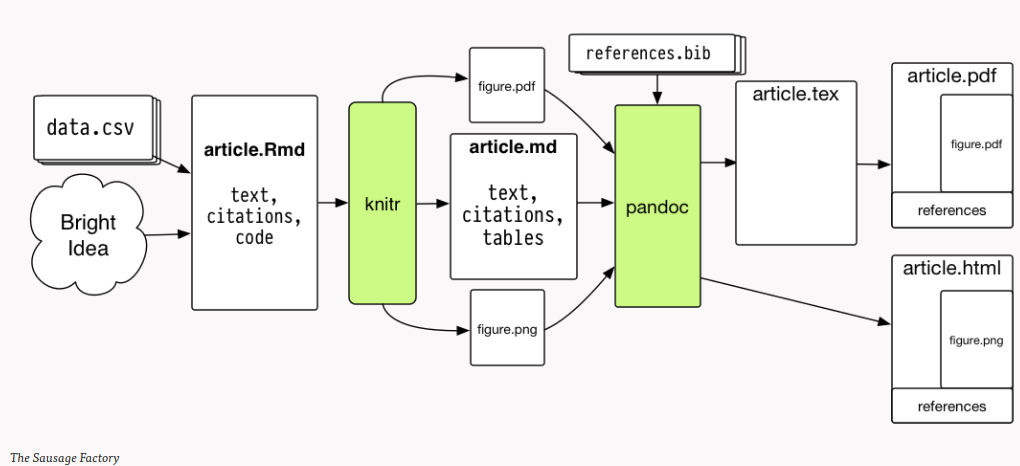
\includegraphics{images/healeysworkflow.png}

El documento central de trabajo es uno en formato .Rmd (Rmarkdown), que combina texto en Markdown y código R, lo que se detalla más abajo. La librería \texttt{Knitr} hace la transformación de este documento a formatos como html y/o pdf, para lo cual utiliza el convertidor pandoc.

No es necesario conocer al detalle todos los elementos de este flujo para hacer funcionar un documento dinámico, sino básicamente dos: 1) Markdown, y 2) Trozos de código. Vamos por parte.

\hypertarget{trozos-chunks-de-cuxf3digo}{%
\subsubsection{Trozos (chunks) de código}\label{trozos-chunks-de-cuxf3digo}}

La caracteristica principal de \texttt{Knitr} es que identifica las secciones de código en la hoja y los ejecuta mediante R. Estos trozos de código se encuentran delimitados de la siguiente manera:

\begin{verbatim}
```{r}
    4+5
```
\end{verbatim}

Es decir, todo lo que comience por \texttt{\textasciigrave{}\textasciigrave{}\textasciigrave{}r} y termine con \texttt{\textasciigrave{}\textasciigrave{}\textasciigrave{}} será identificado como código de análisis (el atajo para generar un chunk en RStudio es \texttt{ctrl+alt+i})

\hypertarget{tipos-de-chunks}{%
\subsubsection{Tipos de chunks}\label{tipos-de-chunks}}

En general hay cinco opciones básicas de edición relacionadas con chunks y su visualización en el documento final. Esto se maneja mediante opciones que aparecen al inicio en el chunk, luego de la letra \texttt{r}

\begin{enumerate}
\def\labelenumi{\arabic{enumi}.}
\tightlist
\item
  código y resultado (opción por defecto)
\end{enumerate}

\begin{verbatim}
```{r}
1 + 1
```
\end{verbatim}

Resulta

\begin{Shaded}
\begin{Highlighting}[]
\DecValTok{1} \OperatorTok{+}\StringTok{ }\DecValTok{1}
\end{Highlighting}
\end{Shaded}

\begin{verbatim}
## [1] 2
\end{verbatim}

\begin{enumerate}
\def\labelenumi{\arabic{enumi}.}
\setcounter{enumi}{1}
\tightlist
\item
  solo código, ocultando resultados:
\end{enumerate}

\begin{verbatim}
```{r, results='hide'}
1 + 1
```
\end{verbatim}

Resulta:

\begin{Shaded}
\begin{Highlighting}[]
\DecValTok{1} \OperatorTok{+}\StringTok{ }\DecValTok{1}
\end{Highlighting}
\end{Shaded}

\begin{enumerate}
\def\labelenumi{\arabic{enumi}.}
\setcounter{enumi}{2}
\tightlist
\item
  solo resultado
\end{enumerate}

\begin{verbatim}
```{r, echo=FALSE}
1 + 1
```
\end{verbatim}

Resulta:

\begin{verbatim}
## [1] 2
\end{verbatim}

\begin{enumerate}
\def\labelenumi{\arabic{enumi}.}
\setcounter{enumi}{3}
\tightlist
\item
  ni código ni resultado \texttt{\{r\ echo=FALSE\ results=\textquotesingle{}hide\textquotesingle{}\}}
\item
  resultado ``tal cual como es'': \texttt{\{r\ results=\textquotesingle{}asis\textquotesingle{}\}} se utiliza principalmente para comandos de generación de tablas, que arrojan un código que luego puede ser interpretado por otro lenguaje (por ejemplo, html)
\end{enumerate}

\hypertarget{trabajando-con-documentos-dinuxe1micos-en-rstudio}{%
\subsection{Trabajando con documentos dinámicos en RStudio}\label{trabajando-con-documentos-dinuxe1micos-en-rstudio}}

RStudio es principalmente un editor para análisis de datos con R, pero últimamente ha ido incorporando herramientas para reportes dinámicos. Para ello utiliza un tipo de archivos con extensión \texttt{Rmd} que significa Rmarkdown. Y en este contexto Rmarkdown es la forma en que Rstudio identifica los archivos que combinan texto y código.

Para generar un archivo Rmarkdown, simplemente new file \textgreater{} Rmarkdown

\includegraphics{images/rmarkdown.gif}

Y luego para convertir este documento, presionar el boton \texttt{Knitr}.

El generador de documentos por defecto trae un texto de ejemplo donde hay analisis y tablas, y además dos cosas:

\begin{itemize}
\item
  \textbf{Preámbulo o YAML (Yet Another Markdown Language)}: esta sección del inicio que se encuentra enmarcada entre \texttt{-\/-\/-} incluye algunos datos básicos del documento que luego se consideran al momento de convertirlo al documento editado final. Por ejemplo, si se prefiere que la conversión sea a html, se incluye la opción \texttt{output:\ html\_document}

\begin{verbatim}
---
title: "nuevo"
author: "jc"
date: "5/30/2019"
output: html_document
---
\end{verbatim}
\item
  \textbf{Chunk de opciones generales}: va al inicio del documento, luego del YAML. En general, la que aparece por defecto \texttt{echo=TRUE} se refiere a que se muestren los resultados de los chunks de código.
\end{itemize}

\hypertarget{reproducibilidad}{%
\section{Reproducibilidad}\label{reproducibilidad}}

  \bibliography{book.bib,packages.bib,openscience.bib}

\end{document}
